\newpage
\section{Foundations of the C++ Concurrency Memory Model\cite{PPTTheC19:online,boehm2008foundations}}


Momory model is the guarantee provided by the runtime environment to a 
multithreaded program, regaring the order of memory operations. 
Each level of the environment(e.g. CPU, virtual machine, compiler) might have a different memory model
.The 
correctness of parallel algorithms depends on the memory model.


\texttt{Threads}  are now part of the C++ 11language.
Their behavior must be fully defined so that the same code
 run the same on different environments regardless of the CPU
  (Intel, AMD, ARM, …) or the OS.




Undefined behaviour matters a lot. See the example shown in \ref{lst:e1} . 
The compiler knows x is bound between 0 and 2, so instead of 
creating a series of if’s, it can simply jump to 
(switch base address + x * constant). 
But if x is shared and unprotected, it might be changed 
between the if and the switch, causing an unrestricted jump,
 which can cause unpredictable damages.
Races are forbidden because the compiler can’t always recognize them (static analysis in not required by the standard), 
and to avoid them the programmer must help the compiler.
In the example above, even if x were somehow protected, it could still be modified between the if and the switch. 
This would have caused the code to behave differently from the serial implementation. 
However, had the compiler known x might be modified by another thread, 
it would not have used the unsafe jump table optimization.


\begin{lstlisting}[language=C,frame=single, caption=An simple example  ,label = lst:e1]
if(x >= 0 && x < 3){
    switch(x){
        case 0 : do0(); break;
        case 1 : do1(); break;
        case 2 : do2(); break;
    }
}
\end{lstlisting}


Single-threaded programs are fairly easy to optimize, because there’s no “external viewer” (other than the output). 
So most of the time they execute “atomically”. Shared variables, however, might be viewed by different threads at 
(almost) any given moment. So, their modifications by one thread must seem to be ordered to other threads.
The listed optimizations in Listing\ref{lst:e1}  are just an example  obviously there are many more.
Notice that in c++11 some optimizations can be seen by other threads, which is fully defined by c++11’s memory model.


A memory location does not depend on the size of the type, and can be part of an array or struct/class.
Bit fields are different: several might occupy a single memory location.
About the example in  Listing\ref{lst:e2}: writing single bytes can be inefficient on some systems.
 It could be faster to read the whole array of chars, for instance, as a single 32-bit word,
  update one element, and write the whole word back. But that might introduce a race on the other elements!
This is similar to having two variables on the same cache line. Updating one must not override an update 
of the other. This requires non-trivial synchronization, and a performance overhead. 
This wasn’t a problem on single threaded programs.
In Java, update of a variable smaller or equal to a dword should not affect an adjacent variable (like C++11). 
However, longs and doubles are not guaranteed to be atomic (unless defined as volatile, in which 
case they are always atomic). This is due to the fact that it is a multi-step operation at the machine code level.
Note: int i:3 means that the compiler will use 3 bits to store i.


\begin{lstlisting}[language=C,frame=single, caption=An simple example  ,label = lst:e2]

struct s {
char c[4];
int i: 3, j: 4;
struct in {
double d;
} id;
};
\end{lstlisting}

The Sequence Before is the order imposed by the appearance of (most) statements in the code, for a single thread.
On some occasions, the sequence of execution is not specified (such as function argument evaluation). 
This cases are therefore unordered with respect to each other. For instance, in f(h(), g()) 
it is unspecified whether h() or g() will be executed first. Yet, both h() and g() are always sequenced 
before f().

Synchronized with is the order imposed by an atomic read of a value that has been atomically written
 by some other thread. The said synchronization does not rely on any synchronization object. 
 It means that when E1 synchronizes with E2, every write done before E1 should be visible 
 to reads done after E2; and no write done after E1 should be visible to reads done before E2. 
 This defines an order that crosses thread boundaries.

 Inter-thread happens-before is a combination of sequenced before and synchronized with.


 Here \ref{fig:p224}, the events in thread 1 inter-thread happen-before the events in thread 2.

 \begin{figure}[H]
    \centering
    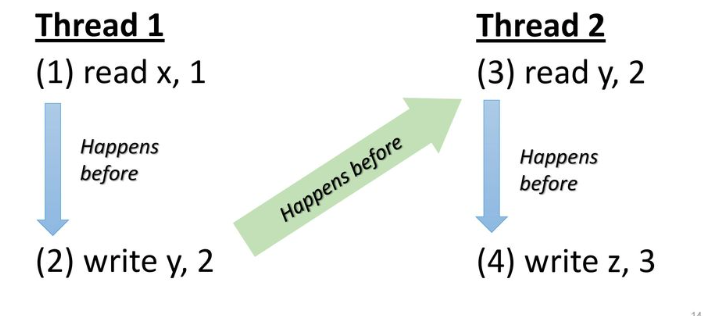
\includegraphics[width=0.4\textwidth]{p224.png}
    \caption{}
    \label{fig:p224}
\end{figure}




The blue arrows \ref{fig:p225} are sequenced-before. The green arrow is synchronized-with. 
Together they form an inter-thread happens-before relation, 
which guarantees the write to y happens-before reading it.
Note that y isn’t atomic, and in general not safe to use as shared variable. 
However, in this particular scenario, its accesses are synchronized by the use of the atomic x.
The assert is guaranteed not to fail

\begin{figure}[H]
    \centering
    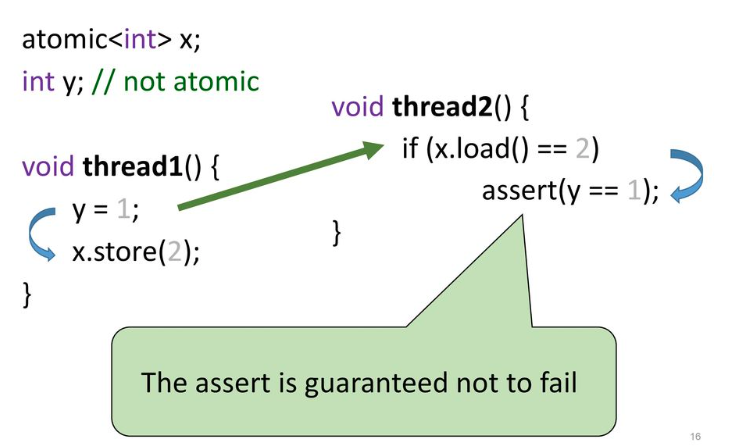
\includegraphics[width=0.4\textwidth]{p225.png}
    \caption{}
    \label{fig:p225}
\end{figure}


Synchronized-with relation exists only between the releasing thread and the acquiring thread
Other threads might see updates in a different order.
All writes before a release are visible after an acquire.
Even if they were relaxed or non-atomic.
Similar to release consistency memory model.






The writes are on different threads. Each acquiring thread is synchronized with 
the thread that has done the release. Thus, the releases are unordered.
If sequential consistency had been used instead of acquire-release,
 the results would have been different. 
 There would have been a total order of writes, so if one of the asserts had succeeded, 
 the other must have failed.

 \begin{figure}[H]
    \centering
    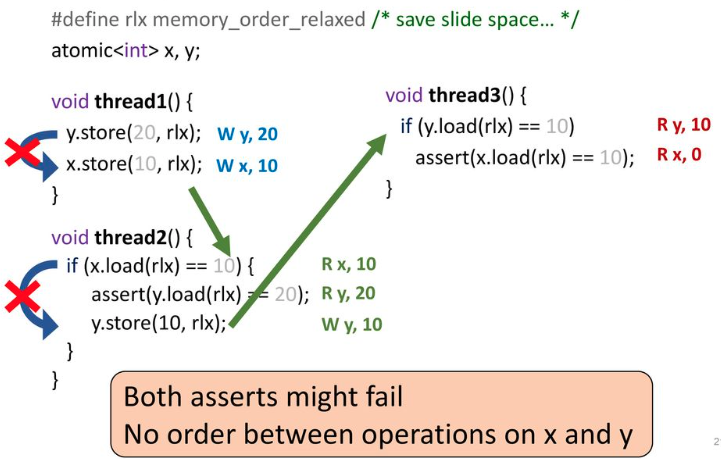
\includegraphics[width=0.4\textwidth]{p226.png}
    \caption{}
    \label{fig:p226}
\end{figure}




In this model, two processors might see writes to two variables(done by some third processor) 
in a different order.
This is where C++ atomic differs from Java volatile: Java never relaxes program order between 
volatile variables, while C++ allows reordering of (and across) atomic variables.



\begin{figure}[H]
    \centering
    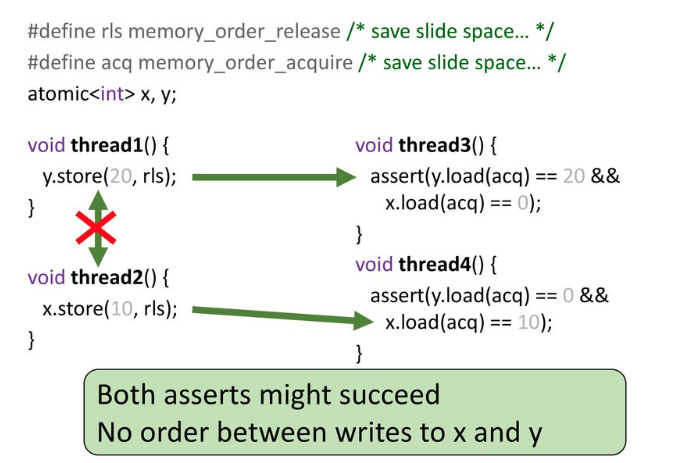
\includegraphics[width=0.4\textwidth]{p227.png}
    \caption{}
    \label{fig:p227}
\end{figure}

Both asserts might fail because the stores on thread 1 are not ordered,
 and different threads might see them in a different order. 
 One way for this to happen is if thread 3 has a speculative load of x before 
 the if. When this is the case, x might be read before threads 1 and 2 
 started to execute.




Predates C++ multi-threading
Serves different purpose
Intended for reading from memory that was written by a device
Does not guarantee atomic
Unspecified memory order
However Java (and C#) volatile is very similar to C++ atomic
volatile was actually the only option in pre-C++11 code, but other than avoiding the use of a register it has no multi-threading semantics, because it was introduced way before C++ supported multi-threading. It does usually do the trick, but not due to some standard guarantee.
Some compilers (VS) add ordering semantics (release consistency) on certain CPUs (Itanium) as an extension – but we’re talking about standard C++ here.


Lock-free code is hard to write
Unless speed is crucial, better use mutexes
Sequential consistency is the default
It is also the memory model for function that does not have memory-model as an input parameter
Use the default sequential consistency and avoid data races. Really.
Acquire-release is hard
Relaxed is much harder
Mixing orders is insane (but allowed)

27 Summary and recommendations (2)
The memory model can be passed as run-time parameter
But it is better to use it as a compilation constant to allow optimizations
We only covered main orders
C++11’s basic features are fully supported by all common compilers.


The memory model, or memory consistency model, specifies the
values that a shared variable read in a multithreaded program is allowed to return. 
The memory model clearly affects programmability. 
It also affects performance and portability by constraining the
transformations that any part of the system may perform. 





A memory model, a.k.a memory consistency model, is a 
specification of the allowed behavior of multithreaded 
programs executing with shared memory . 
The most basic model is sequential consistency (SC), 
where all insructions from all threads (appear to) form a
 total order that is consistent with the program order on 
 each thread.



\subsection{Concurrency needs sync }

For performance gains, modern CPUs often execute 
instructions out of order to fully utilize resources.
 Since the hardware enforces instructions integrity,
  we can never notice this in a single thread execution. 
  However, for multiple threads, this can lead to 
  unpredictable bahaviors.

In multi-threaded execution, uncontrolled scheduling leads 
to data race, where results depend on the timing execution 
of the code. With some bad luck (i.e., context switches 
that occur at untimely points in the execution), we get 
the wrong result.

\subsubsection{mutual exclusion (atomic)}
To achieve atomicity, we can ask hardware for a few useful instructions to build mutual exclusion, which guarantees that if one thread is executing within the critical section, the others will be prevented from doing so.

\subsubsection{ waiting for another (conditional variable)}
There are many cases where a thread continues its execution 
only when some condition is met. Thus, one thread must wait
 for another to complete some action before it continues. 

\subsection{Low-Level Atomics}

